\documentclass[12pt]{report}
\usepackage[utf8]{inputenc}
\usepackage[russian]{babel}
%\usepackage[14pt]{extsizes}
\usepackage{listings}
\usepackage{graphicx}
\usepackage{amsmath,amsfonts,amssymb,amsthm,mathtools} 
\usepackage{pgfplots}
\usepackage{filecontents}
\usepackage{indentfirst}
\usepackage{eucal}
\usepackage{float} 
\usepackage{amsmath}
\usepackage{enumitem}
\usepackage[justification=centering]{caption} 
\usepackage{tikz}
\usepackage{pgfplots}
\pgfplotsset{compat=newest}

\frenchspacing

\usepackage{indentfirst} % Красная строка


%\usetikzlibrary{datavisualization}
%\usetikzlibrary{datavisualization.formats.functions}

\usepackage{amsmath}


% Для листинга кода:
\lstset{ %
	language=haskell,                 % выбор языка для подсветки (здесь это С)
	basicstyle=\small\sffamily, % размер и начертание шрифта для подсветки кода
	numbers=left,               % где поставить нумерацию строк (слева\справа)
	numberstyle=\tiny,           % размер шрифта для номеров строк
	stepnumber=1,                   % размер шага между двумя номерами строк
	numbersep=5pt,                % как далеко отстоят номера строк от подсвечиваемого кода
	showspaces=false,            % показывать или нет пробелы специальными отступами
	showstringspaces=false,      % показывать или нет пробелы в строках
	showtabs=false,             % показывать или нет табуляцию в строках
	frame=single,              % рисовать рамку вокруг кода
	tabsize=2,                 % размер табуляции по умолчанию равен 2 пробелам
	captionpos=t,              % позиция заголовка вверху [t] или внизу [b] 
	breaklines=true,           % автоматически переносить строки (да\нет)
	breakatwhitespace=false, % переносить строки только если есть пробел
	escapeinside={\#*}{*)}   % если нужно добавить комментарии в коде
}

\usepackage[left=2cm,right=2cm, top=2cm,bottom=2cm,bindingoffset=0cm]{geometry}

\usepackage{listings}

\usepackage{titlesec}
\titleformat{\section}
{\normalsize\bfseries}
{\thesection}
{1em}{}
\titlespacing*{\chapter}{0pt}{-30pt}{8pt}
\titlespacing*{\section}{\parindent}{*4}{*4}
\titlespacing*{\subsection}{\parindent}{*4}{*4}
\usepackage{setspace}

\titleformat{\chapter}{\LARGE\bfseries}{\thechapter}{20pt}{\large\bfseries}
\titleformat{\section}{\Large\bfseries}{\thesection}{20pt}{\large\bfseries}

\makeatletter 

\begin{document}
	
%\def\chaptername{} % убирает "Глава"
\thispagestyle{empty}
\begin{titlepage}
	\noindent \begin{minipage}{0.15\textwidth}
		
\includegraphics[width=\linewidth]{pics/logo}
	\end{minipage}
	\noindent\begin{minipage}{0.9\textwidth}\centering
		\textbf{Министерство науки и высшего образования Российской Федерации}\\
		\textbf{Федеральное государственное бюджетное образовательное учреждение высшего образования}\\
		\textbf{~~~«Московский государственный технический университет имени Н.Э.~Баумана}\\
		\textbf{(национальный исследовательский университет)»}\\
		\textbf{(МГТУ им. Н.Э.~Баумана)}
	\end{minipage}
	
	\noindent\rule{18cm}{3pt}
	\newline\newline
	\noindent ФАКУЛЬТЕТ $\underline{\text{«Информатика и системы управления»}}$ \newline\newline
	\noindent КАФЕДРА $\underline{\text{«Программное обеспечение ЭВМ и информационные технологии»}}$\newline\newline\newline\newline\newline
	
	
	\begin{center}
		\noindent\begin{minipage}{1.3\textwidth}\centering
			\Large\textbf{  Отчёт по лабораторной работе №11-12 по курсу}\newline\newline
			\textbf{<<Функциональное и логическое}\newline
			\textbf{\indent\indent\indent программирование>>}\newline
		\end{minipage}
	\end{center}
	
	~\\\\\\\\\\\\
	\large
	\noindent\textbf{Тема } $\underline{\text{Структурные программы на Prolog. Работа программы на Prolog.}}$\newline\newline
	\noindent\textbf{Студент } $\underline{\text{Сироткина П.Ю.}}$\newline\newline
	\noindent\textbf{Группа } $\underline{\text{ИУ7-66Б}}$\newline\newline
	\noindent\textbf{Преподаватели } $\underline{\text{Толпинская Н.Б., Строганов Ю.В.}}$\newline\newline\newline
	
	\begin{center}
		\vfill
		Москва~---~\the\year
		~г.
	\end{center}
\end{titlepage}

\chapter*{Лабораторная работа №11}
\section*{Часть 1}

Разработать свою программу - «Телефонный справочник». Протестировать работу программы.

\begin{lstlisting}
domains
		name, phone_number = symbol.

predicates
		phone(name, phone_number)  

clauses
		phone("Polina", "111").
		phone("Polina", "222").
		phone("Anna",   "333").
		phone("Ivan",   "444").
		phone("Petr",   "555").
		phone("Petr",   "666").

goal
		%phone(Name, "111").
		% Name = Polina
		% 1 Solution

		%phone("Polina", Phone_number).
		% Phone_number = 111
		% Phone_number = 222
		% 2 Solutions

		phone("Ivan", Phone_number).
		% Phone_number = 444
		% 1 Solution
\end{lstlisting}

\section*{Часть 2}

Составить программу – базу знаний, с помощью которой можно определить, например, множество студентов, обучающихся в одном ВУЗе и их телефоны. Студент может одновременно обучаться в нескольких ВУЗах. Привести примеры возможных вариантов вопросов и варианты ответов (не менее 3-х). Описать порядок формирования вариантов
ответа.

Исходную базу знаний сформировать с помощью только фактов.

*Исходную базу знаний сформировать, используя правила.

**Разработать свою базу знаний (содержание произвольно).

(См. след. лист)

\clearpage

\begin{lstlisting}
domains
		student_id, university_id = integer.
		name, phone_number, university_name = symbol.

predicates
		student_info(student_id, name, phone_number)
		university_info(university_id, university_name)
		study(student_id, university_id)
		students_from(university_id, name, phone_number)

clauses
		student_info(0, "Polina", "111").
		student_info(0, "Polina", "112").
		student_info(1, "Anna",   "222").
		student_info(2, "Ivan",   "333").
		
		university_info(0, "BMSTU").
		university_info(1, "MSU").
		university_info(2, "HSE").
		
		study(0, 1).
		study(1, 0).
		study(1, 1).
		study(2, 2).
		
		students_from(University_id, Name, Phone_number) :- student_info(Student_id, Name, Phone_number), study(Student_id, University_id).

goal
		students_from(1, Name, Phone_number).
		% Name = Polina, Phone_number = 111
		% Name = Polina, Phone_number = 112
		% Name = Anna, Phone_number = 222
		% 3 Solution
		
		%students_from(University_id, Name, "333").
		% University_id = 2, Name = Ivan
		% 1 Solution
		
		%students_from(University_id, "Anna", Phone_number).
		% University_id = 0, Phone_number = 222
		% University_id = 1, Phone_number = 222
		% 2 Solutions
\end{lstlisting}

\chapter*{Лабораторная работа №12}

\section*{Часть 1}

Составить программу, т.е. модель предметной области – базу знаний, объединив в ней информацию – знания:
\begin{itemize}
	\item «Телефонный справочник»: Фамилия, №тел, Адрес – структура (Го-
	род, Улица, №дома, №кв);
	\item «Автомобили»: Фамилия\_владельца, Марка, Цвет, Стоимость, и др.;
	\item «Вкладчики банков»: Фамилия, Банк, счет, сумма, др;
\end{itemize} 

Владелец может иметь несколько телефонов, автомобилей, вкладов (Фак-
ты). 

Используя правила, обеспечить возможность поиска:
\begin{enumerate}
	\item \begin{itemize}
		\item По № телефона найти: Фамилию, Марку автомобиля, Стоимость
		автомобиля (может быть несколько);
		\item Используя сформированное в пункте а) правило, по № телефона найти: только Марку автомобиля (автомобилей может быть несколько).
	\end{itemize}
	\item Используя простой, не составной вопрос: по Фамилии (уникальна в
	городе, но в разных городах есть однофамильцы) и Городу проживания найти: Улицу проживания, Банки, в которых есть вклады и №телефона.
\end{enumerate}

Для одного из вариантов ответов, и для а) и для б), описать словесно
порядок поиска ответа на вопрос, указав, как выбираются знания, и, при
этом, для каждого этапа унификации, выписать подстановку – наибольший
общий унификатор, и соответствующие примеры термов.

\begin{lstlisting}
	domains
			surname, phone = symbol.
			city, street = symbol.
			house, flat = integer.
			address = address_struct(city, street, house, flat)
			mark, color = symbol.
			cost = integer.
			bank = symbol.
			account, sum = integer.
	
	predicates
			has_phone(surname, phone, address)
			has_car(surname, mark, color, cost)
			has_deposite(surname, bank, account, sum)
	
			info_by_phone(phone, surname, mark, cost)
			only_mark_by_phone(phone, mark)
			info_by_surname_and_city(surname, city, street, bank, phone)
	
	clauses
			has_phone("Petrov", "111",  address_struct("Moscow",     "Gagarina", 1, 1)).
			has_phone("Petrov", "222",  address_struct("Moscow",     "Gagarina", 1, 1)).
			has_phone("Ivanov", "333",  address_struct("Vladimir",   "Lenina", 2, 2)).
			has_phone("Volkov", "444",  address_struct("Sevastopol", "Lenina", 2, 2)).
			has_phone("Sidorov", "555", address_struct("Kazan",      "Lomonosova", 3, 3)).
			
			has_car("Petrov", "BMW",  "black", 1000).
			has_car("Ivanov", "Audi", "black", 1500).
			has_car("Ivanov", "Audi", "white", 1500).
			has_car("Volkov", "Lada", "white", 500).
			
			has_deposite("Petrov",  "Alpha", 0, 5000).
			has_deposite("Ivanov",  "Beta",  1, 5500).
			has_deposite("Volkov",  "Gamma", 2, 6000).
			has_deposite("Sidorov", "Alpha", 3, 6500).
			has_deposite("Sidorov", "Beta",  4, 7000).
			
			info_by_phone(Phone, Surname, Mark, Cost) :- has_phone(Surname, Phone, _), has_car(Surname, Mark, _, Cost).
			only_mark_by_phone(Phone, Mark) :- info_by_phone(Phone, _, Mark, _).
			info_by_surname_and_city(Surname, City, Street, Bank, Phone) :- has_phone(Surname, Phone, address_struct(City, Street, _, _)), has_deposite(Surname, Bank, _, _).
	
	goal
			%info_by_phone("444", Surname, Mark, Cost).
			% Surname = Volkov, Mark = Lada, Cost = 500
			% 1 Solution
			
			%only_mark_by_phone("333", Mark).
			% Mark = Audi
			% Mark = Audi
			% 2 Solutions
			
			info_by_surname_and_city("Sidorov", "Kazan", Street, Bank, Phone).
			% Street = Lomonosova, Bank = Alpha, Phone = 555
			% Street = Lomonosova, Bank = Beta, Phone = 555
			% 2 Solutions
\end{lstlisting}

\clearpage
\begin{figure}[!h]
	\center{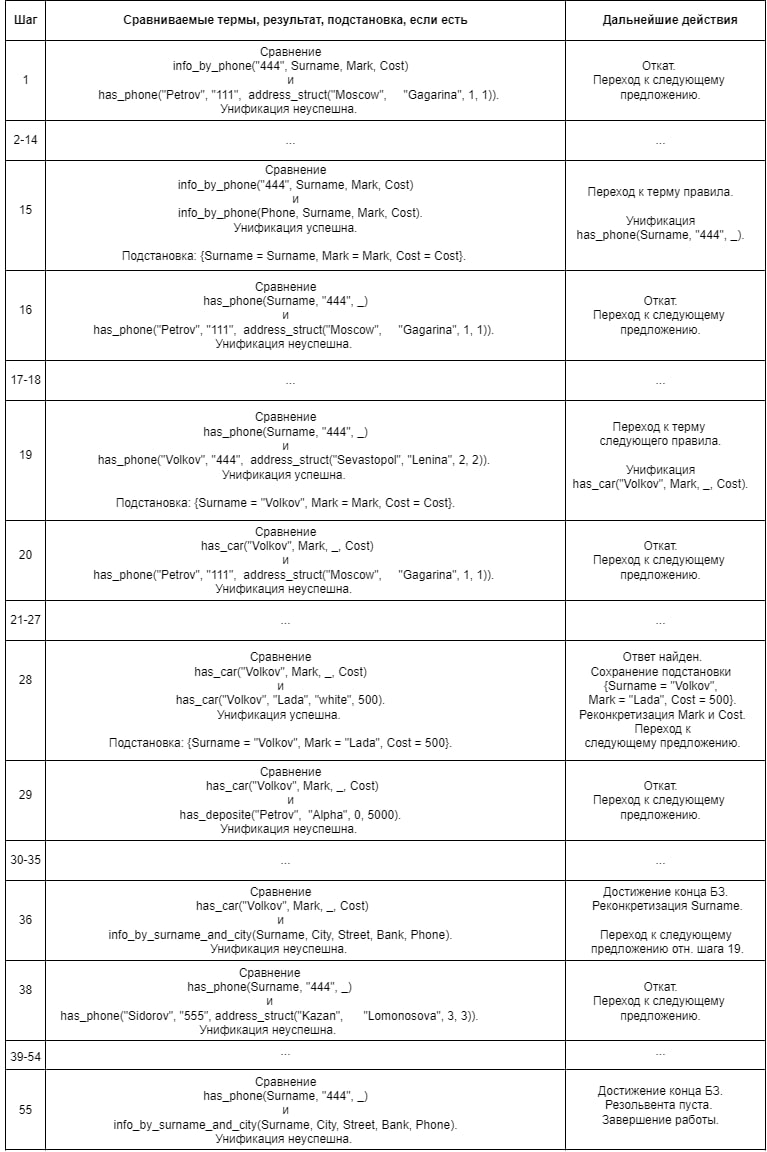
\includegraphics[scale=0.8]{pics/1.jpg}}
\end{figure}

\clearpage
\begin{figure}[!h]
	\center{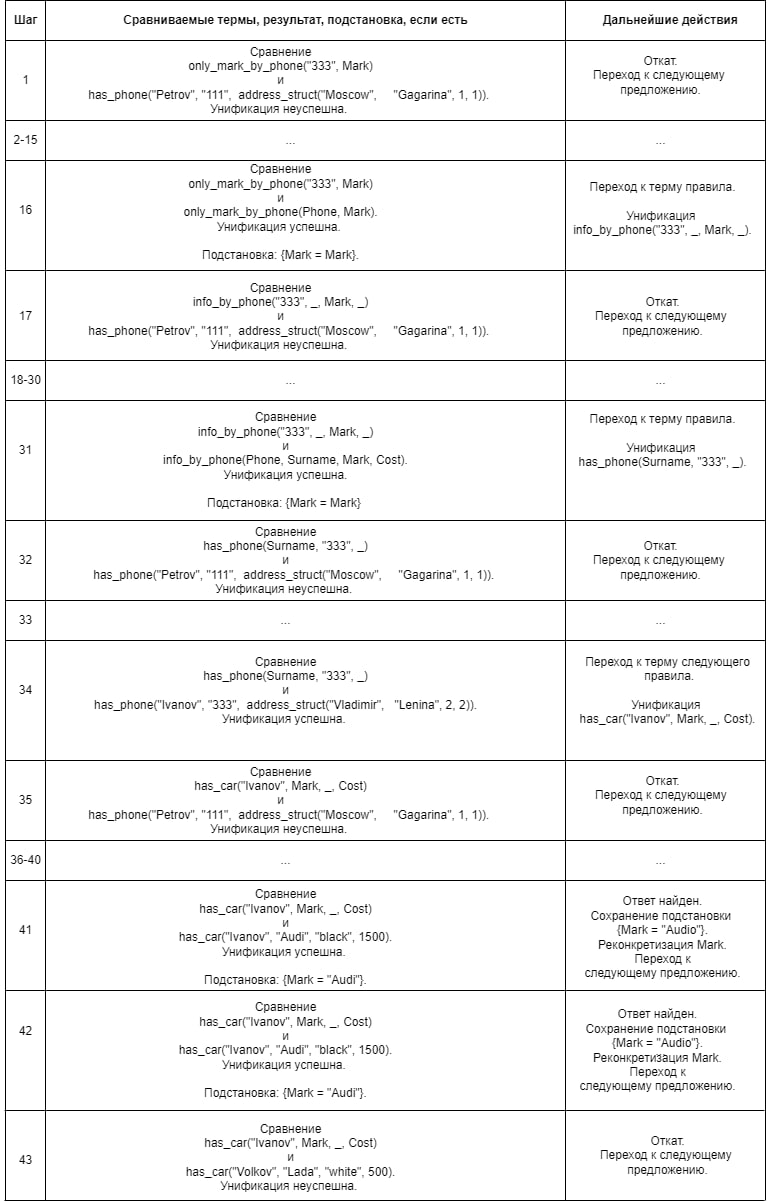
\includegraphics[scale=0.75]{pics/2_1.jpg}}
\end{figure}

\clearpage
\begin{figure}[!h]
	\center{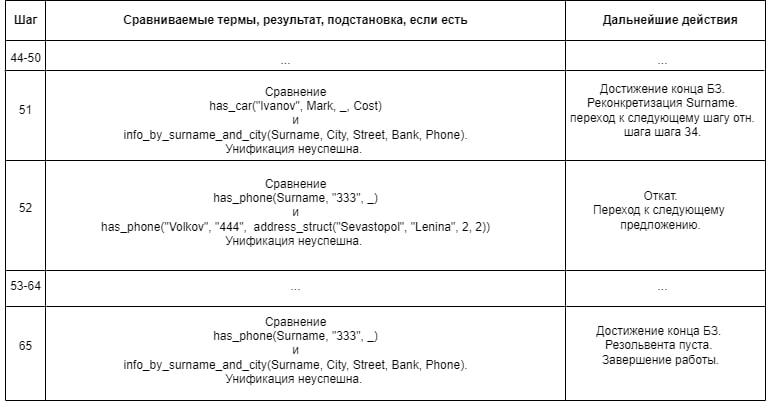
\includegraphics[scale=0.8]{pics/2_2.jpg}}
\end{figure}

\clearpage
\begin{figure}[!h]
	\center{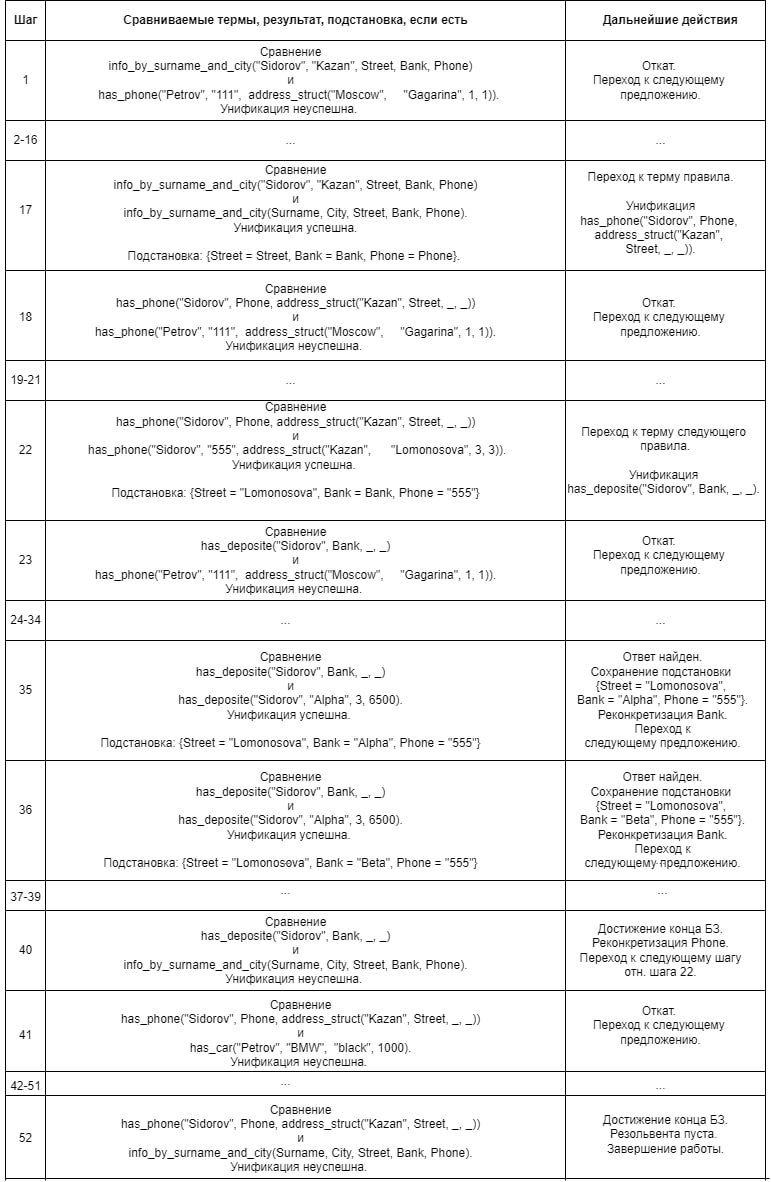
\includegraphics[scale=0.74]{pics/3.jpg}}
\end{figure}

\section*{Часть 2}

Составить программу, объединив в ней информацию-знания (12.1). По Марке и Цвету автомобиля найти Фамилию, Город, Телефон и Банки, в кото-
рых владелец автомобиля имеет вклады. Владельца может быть несколько (не более трех), один и ни одного.

\begin{enumerate}
	\item Для каждого из трех вариантов подробно описать порядок формирования ответа в виде таблицы. При этом указать – отметить моменты очередного запуска алгоритма унификации и полный результат его работы. Обосновать следующий шаг работы системы. Выписать унификаторы – подстановки. Указать моменты, причины и результат
	отката, если он есть.
	\item Для случая нескольких владельцев (2-х). Приведите пример (таблицы) работы системы при разных порядках следования в БЗ процедур,
	и знаний в них («Телефонный справочник», «Автомобили», «Вкладчики банков» или «Автомобили», «Вкладчики банков», «Телефонный
	справочник»). Сделать вывод: одинаковы ли множество работ и объем в разных случаях.
	\item Оформите 2 таблицы, демонстрирующие порядок работы алгоритма
	унификации вопроса и подходящего заголовка правила (для двух случаев из пункта 2) и укажите результаты его работы: ответ и побочный эффект.
\end{enumerate}

\begin{lstlisting}
	domains
			surname, phone = symbol.
			city, street = symbol.
			house, flat = integer.
			address = address_struct(city, street, house, flat)
			mark, color = symbol.
			cost = integer.
			bank = symbol.
			account, sum = integer.
	
	predicates
			has_phone(surname, phone, address)
			has_car(surname, mark, color, cost)
			has_deposite(surname, bank, account, sum)
			
			info_by_phone(phone, surname, mark, cost)
			only_mark_by_phone(phone, mark)
			info_by_surname_and_city(surname, city, street, bank, phone)
			
			info_by_mark_and_color(mark, color, surname, city, phone, bank)
	
	clauses
			has_phone("Petrov",  "111",  address_struct("Moscow",     "Gagarina", 1, 1)).
			has_phone("Ivanov",  "222",  address_struct("Vladimir",   "Lenina", 2, 2)).
			has_phone("Sidorov", "333",  address_struct("Kazan",      "Lomonosova", 3, 3)).
			
			has_car("Petrov", "BMW", "black", 500).
			
			has_car("Ivanov", "Audi", "white", 1500).
			has_car("Petrov", "Audi", "white", 1500).
			
			has_deposite("Petrov", "Alpha", 0, 1000).
			has_deposite("Ivanov", "Gamma", 1, 2000).
			has_deposite("Sidorov", "Beta", 2, 3000).
			
			info_by_phone(Phone, Surname, Mark, Cost) :- has_phone(Surname, Phone, _), has_car(Surname, Mark, _, Cost).
			only_mark_by_phone(Phone, Mark) :- info_by_phone(Phone, _, Mark, _).
			info_by_surname_and_city(Surname, City, Street, Bank, Phone) :- has_phone(Surname, Phone, address_struct(City, Street, _, _)), has_deposite(Surname, Bank, _, _).
			
			info_by_mark_and_color(Mark, Color, Surname, City, Phone, Bank) :- has_car(Surname, Mark, Color, _), has_phone(Surname, Phone, address_struct(City, _, _, _)), has_deposite(Surname, Bank, _, _).
	
	goal
			%info_by_mark_and_color("Lada", "white", Surname, City, Phone, Bank).
			% No solutions
			
			info_by_mark_and_color("BMW", "black", Surname, City, Phone, Bank).
			% Surname = Petrov, City = Moscow, Phone = 111, Bank = Alpha
			% 1 Solution
			
			%info_by_mark_and_color("Audi", "white", Surname, City, Phone, Bank).
			% Surname = Ivanov, City = Vladimir, Phone = 222, Bank = Gamma
			% Surname = Petrov, City = Moscow, Phone = 111, Bank = Alpha
			% 2 Solutions
\end{lstlisting}

\clearpage
\begin{figure}[!h]
	\center{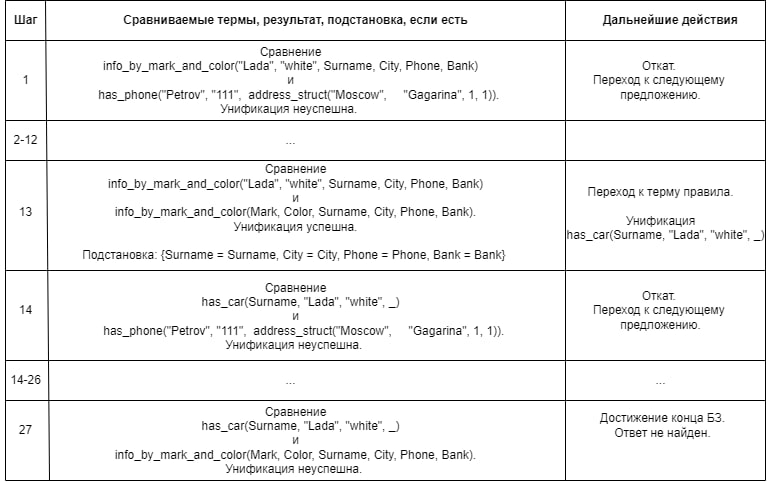
\includegraphics[scale=0.85]{pics/02_1.jpg}}
\end{figure}

\clearpage
\begin{figure}[!h]
	\center{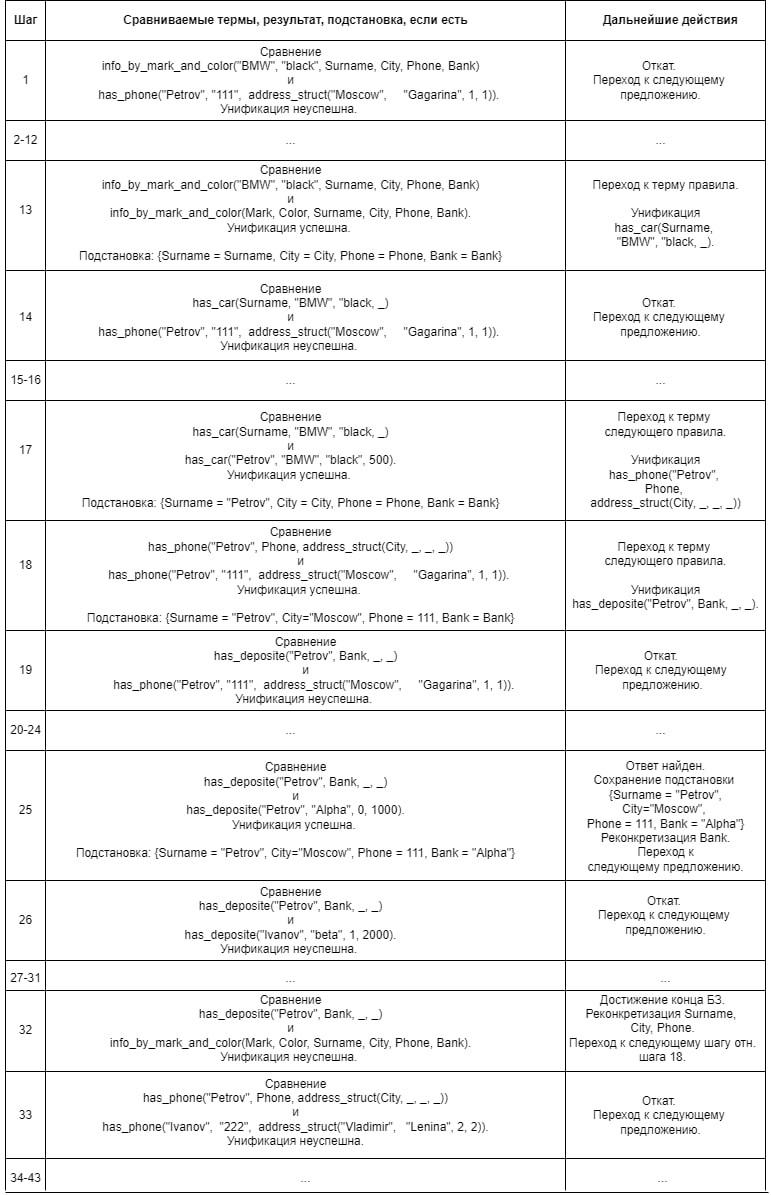
\includegraphics[scale=0.75]{pics/02_2_1.jpg}}
\end{figure}

\clearpage
\begin{figure}[!h]
	\center{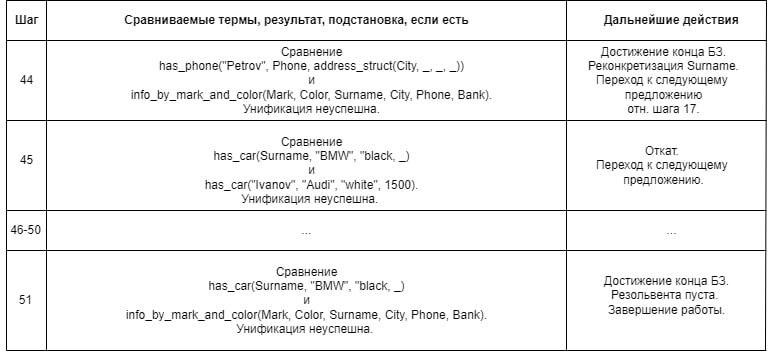
\includegraphics[scale=0.85]{pics/02_2_2.jpg}}
\end{figure}

\clearpage
\begin{figure}[!h]
	\center{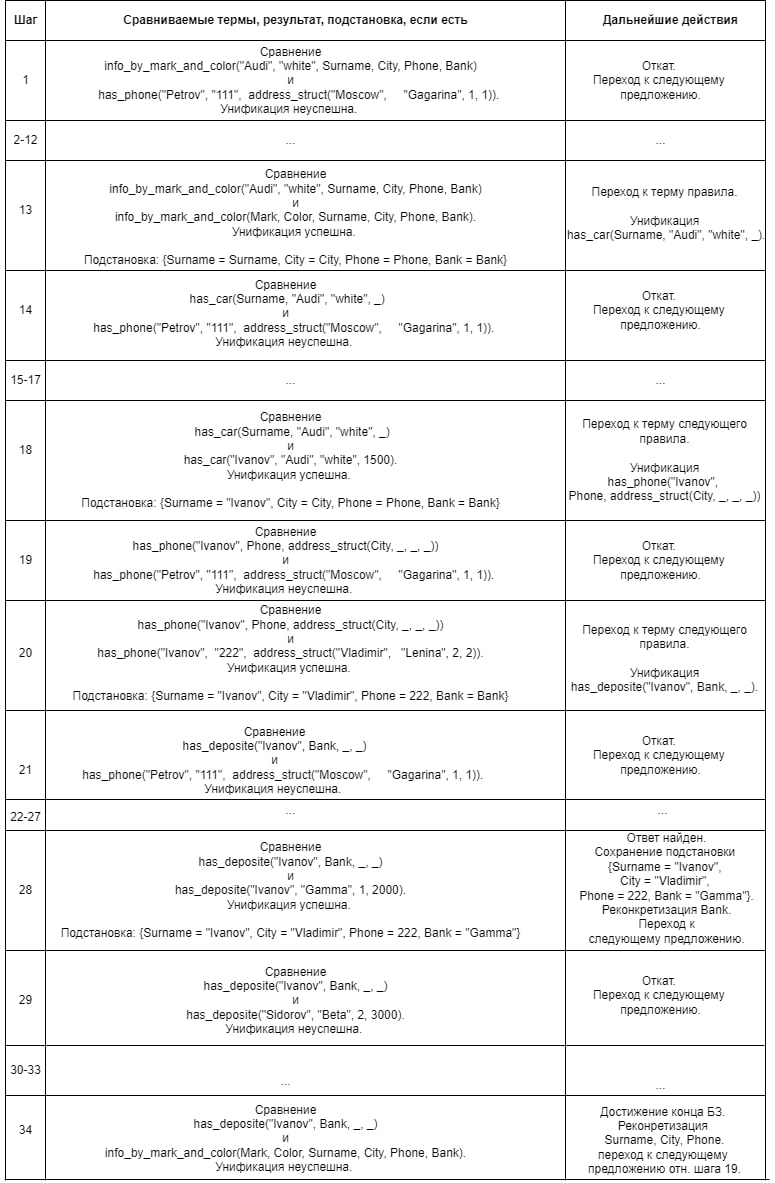
\includegraphics[scale=0.75]{pics/02_3_1.jpg}}
\end{figure}

\clearpage
\begin{figure}[!h]
	\center{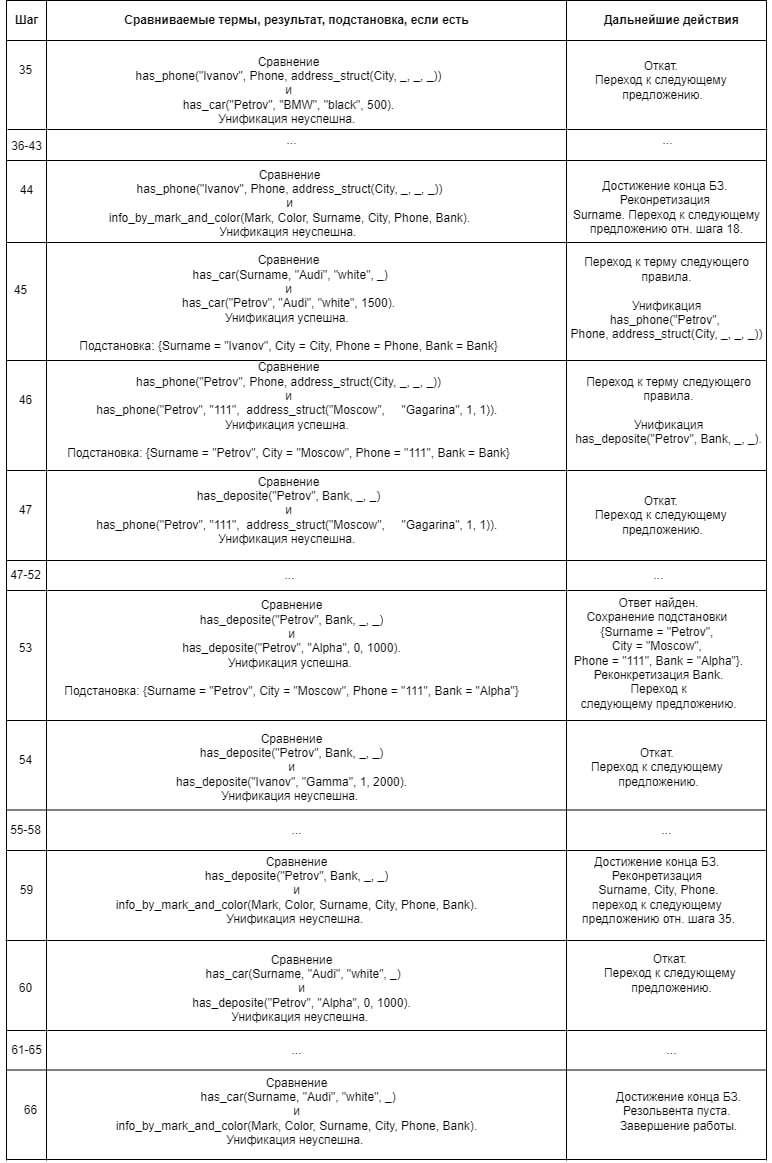
\includegraphics[scale=0.75]{pics/02_3_2.jpg}}
\end{figure}

\clearpage
\begin{figure}[!h]
	\center{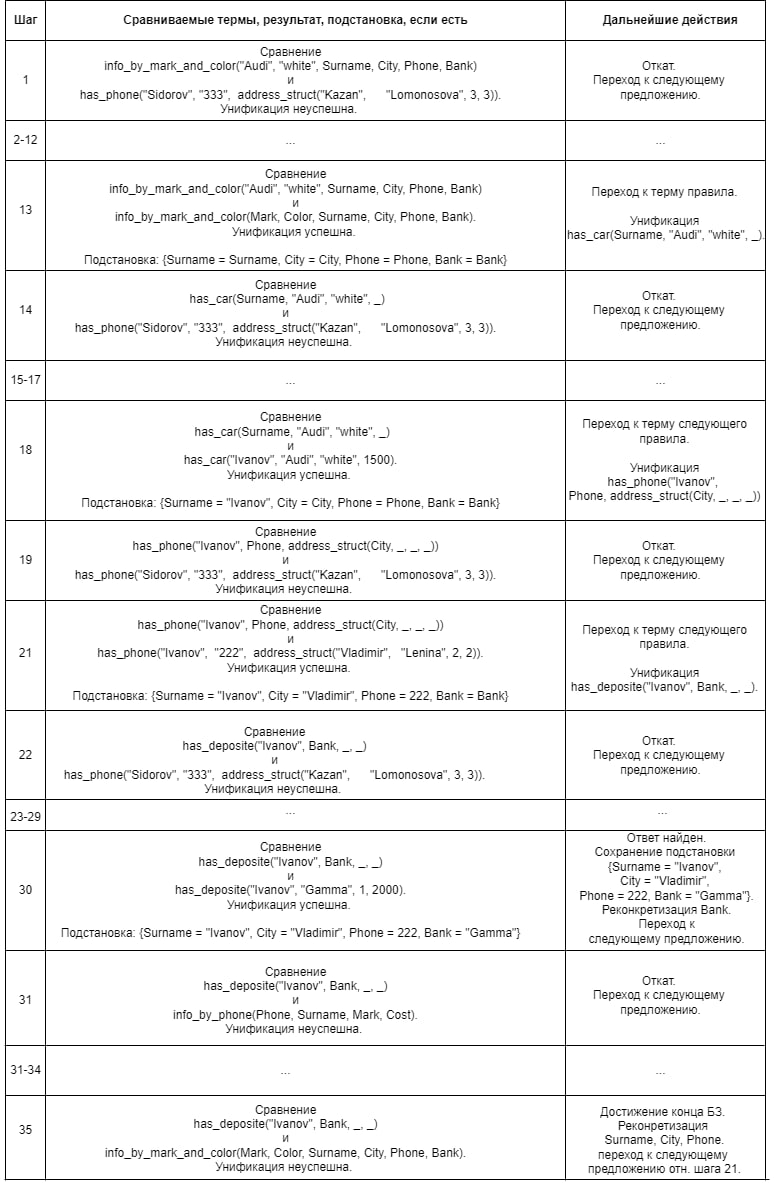
\includegraphics[scale=0.75]{pics/02_4_1.jpg}}
\end{figure}

\clearpage
\begin{figure}[!h]
	\center{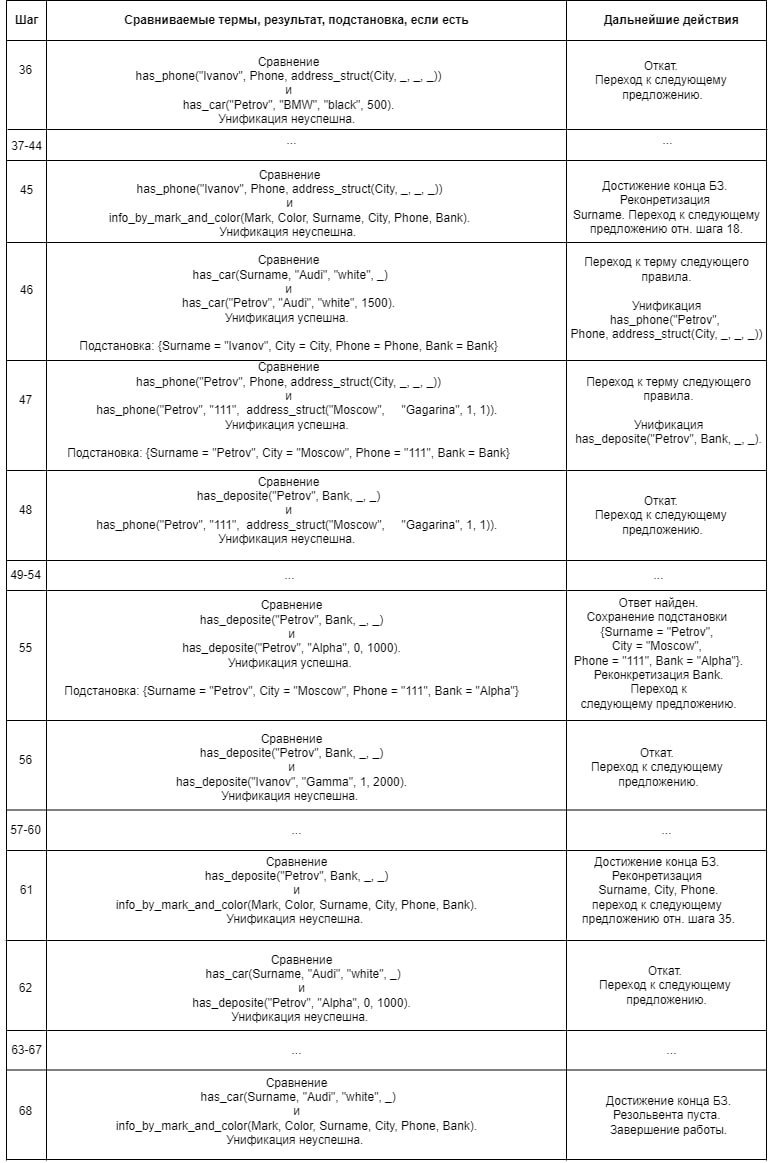
\includegraphics[scale=0.75]{pics/02_4_2.jpg}}
\end{figure}

\end{document}